\section{Results}
\label{sec:results}

\subsection{Historical holdout and initial graph feasibility}

On the 30-question principal holdout, top-down routing reached Hit@5 of 0.767 versus 0.700 for bottom-up dense retrieval. The adaptive method also reached 0.767, but its paired interval against text-only fusion included zero. Graph-constrained text retrieval reached only 0.100, and disabling graph access left adaptive aggregate metrics unchanged.

The graph recovered all six accepted shortage-event paths within five candidates. Text retrieval answered only one of their six accompanying regulatory targets within five. This initial result supported explicit-relation feasibility and motivated a more controlled chain-ranking test.

\subsection{Enrichment ablation}

BM25 led the independent enrichment ablation with Hit@5 of 0.867, MRR of 0.726, and nDCG@5 of 0.662 (\Cref{tab:ablation}). Adding chunk summaries changed little. Generated question profiles reduced MRR by 0.171 and nDCG@5 by 0.167 versus the raw dense index; both paired adjusted tests gave $p=0.024$. Mapping generated items back to source chunks preserved provenance but did not prevent competition for nearest-neighbor positions.

\subsection{Adjudicated evaluation}

The reviewers agreed on 96.7\% of question-status and evidence-completeness labels. Core binary passage agreement was 0.941, with $\kappa=0.792$ (95\% interval [0.718, 0.862]) and AC1$=0.918$ ([0.880, 0.949]). Joint adjudication left no unresolved item.

On the one-shot 58-question run, BM25 achieved Hit@5 of 0.948, MRR of 0.820, and nDCG@5 of 0.800. The selective gate reached 0.897, 0.787, and 0.757, failing its prespecified superiority rule.

\begin{table}[t]
\centering
\begin{threeparttable}
\caption{Independent enrichment ablation ($n=30$; query-bootstrap 95\% confidence intervals).}
\label{tab:ablation}
\small
\begin{tabularx}{\textwidth}{l*{3}{>{\centering\arraybackslash}X}}
\toprule
Method & Hit@5 & MRR & nDCG@5 \\
\midrule
BM25 raw & \textbf{0.867 [0.733, 0.967]} & \textbf{0.726 [0.593, 0.846]} & \textbf{0.662 [0.528, 0.789]} \\
R1: source chunks & 0.733 [0.567, 0.900] & 0.557 [0.412, 0.702] & 0.526 [0.380, 0.673] \\
R2: R1 + chunk summaries & 0.733 [0.567, 0.867] & 0.554 [0.408, 0.703] & 0.524 [0.380, 0.669] \\
R3: R2 + generated questions & 0.567 [0.400, 0.733] & 0.384 [0.253, 0.522] & 0.357 [0.220, 0.502] \\
R4: R3 + table summaries & 0.567 [0.400, 0.733] & 0.384 [0.252, 0.524] & 0.357 [0.217, 0.500] \\
BM25 + R4 RRF & 0.733 [0.567, 0.867] & 0.606 [0.461, 0.747] & 0.508 [0.366, 0.652] \\
Full adaptive & 0.800 [0.667, 0.933] & 0.608 [0.464, 0.747] & 0.571 [0.430, 0.713] \\
\bottomrule
\end{tabularx}
\begin{tablenotes}[flushleft]\footnotesize
\item R1--R4 are cumulative flat dense indexes. Generated representations map back to source chunks before evaluation.
\end{tablenotes}
\end{threeparttable}
\end{table}


\subsection{Neural boundary experiments}

BM25 found Gold within its top 50 for all 58 questions. Qwen3 reranking raised Hit@5 to 0.983, MRR to 0.832, and nDCG@5 to 0.817. The paired differences were 0.034 [0.000, 0.086], 0.012 [-0.082, 0.104], and 0.017 [-0.058, 0.093], respectively. The point estimates improved, but the intervals did not establish a general gain.

MedCPT gave the opposite result. Full-corpus dual-encoder retrieval reached Hit@5 of 0.345, MRR of 0.300, and nDCG@5 of 0.246. MedCPT cross-encoding of BM25's top 50 preserved candidate recall but reduced the three metrics to 0.603, 0.457, and 0.431. All paired 95\% intervals against BM25 were below zero for these metrics. The pattern held across single-clause, table, document-structure, and cross-document slices.

\begin{table}[t]
\centering
\begin{threeparttable}
\caption{Source-chunk retrieval on 58 adjudicated questions.}
\label{tab:final58}
\begin{tabular}{lccc}
\toprule
Method & Hit@5 & MRR & nDCG@5 \\
\midrule
Context-matched BM25 & 0.948 & 0.820 & 0.800 \\
Youtu source-chunk dense & 0.759 & 0.574 & 0.545 \\
Selective table gate & 0.897 & 0.787 & 0.757 \\
Qwen3 over BM25 top 50$^{*}$ & \textbf{0.983} & \textbf{0.832} & \textbf{0.817} \\
MedCPT dual encoder$^{*}$ & 0.345 & 0.300 & 0.246 \\
MedCPT over BM25 top 50$^{*}$ & 0.603 & 0.457 & 0.431 \\
\bottomrule
\end{tabular}
\begin{tablenotes}[flushleft]\footnotesize
\item $^{*}$Feedback-motivated locked extensions on already observed Gold questions. Qwen3 and the MedCPT cross-encoder rerank BM25's frozen top 50; MedCPT dual-encoder retrieval searches all 2,478 chunks.
\end{tablenotes}
\end{threeparttable}
\end{table}


\subsection{Exploratory evidence-chain ranking}

Candidate generation contained the accepted chain for every question. On the 28 audit-qualified questions, R1 achieved exact-chain Hit@1 of 0.571, Hit@3 and Hit@5 of 0.786, and MRR of 0.663 (\Cref{tab:graphchain}). Its Hit@5 difference from M0 was 0.643 [0.464, 0.821]. Removing relation cues reduced Hit@5 to 0.143, whereas removing orientation reduced it to 0.750; the R1--direction-off difference was 0.036 [-0.071, 0.143]. Thus most measured gain came from matching relation phrases rather than the orientation term.

Performance varied sharply by task. R1 recovered all shortage chains within one candidate and reached Hit@5 of 0.900 on regulatory logic, but only 0.375 on the eight retained API-supply questions. The transparent 30-question analysis, which includes the two ambiguous questions, gave Hit@5 of 0.733 and MRR of 0.626. Twelve queries reached the deterministic 50,000-candidate cap, but none aborted or lacked an anchor.

\begin{table}[!ht]
\centering
\begin{threeparttable}
\caption{Exact evidence-chain ranking on 28 audit-qualified questions.}
\label{tab:graphchain}
\small
\begin{tabular}{lcccc}
\toprule
Method & Hit@1 & Hit@3 & Hit@5 & MRR \\
\midrule
B0: untyped traversal & 0.000 & 0.036 & 0.179 & 0.067 \\
M0: relation-blind matched & 0.036 & 0.107 & 0.143 & 0.140 \\
Cue-off & 0.036 & 0.071 & 0.143 & 0.180 \\
Direction-off & 0.500 & 0.714 & 0.750 & 0.600 \\
R1: relation-aware & \textbf{0.571} & \textbf{0.786} & \textbf{0.786} & \textbf{0.663} \\
\bottomrule
\end{tabular}
\begin{tablenotes}[flushleft]\footnotesize
\item Questions were constructed from known graph relations. Two ambiguous API questions were retained in the audit ledger but excluded from strict metrics; the unfiltered 30-question R1 Hit@5 was 0.733.
\end{tablenotes}
\end{threeparttable}
\end{table}


\Cref{fig:retrieval-findings} consolidates the principal text-retrieval boundary, graph-chain ablation, and task-specific failure pattern in a common Hit@5 view.

\begin{figure}[!t]
  \centering
  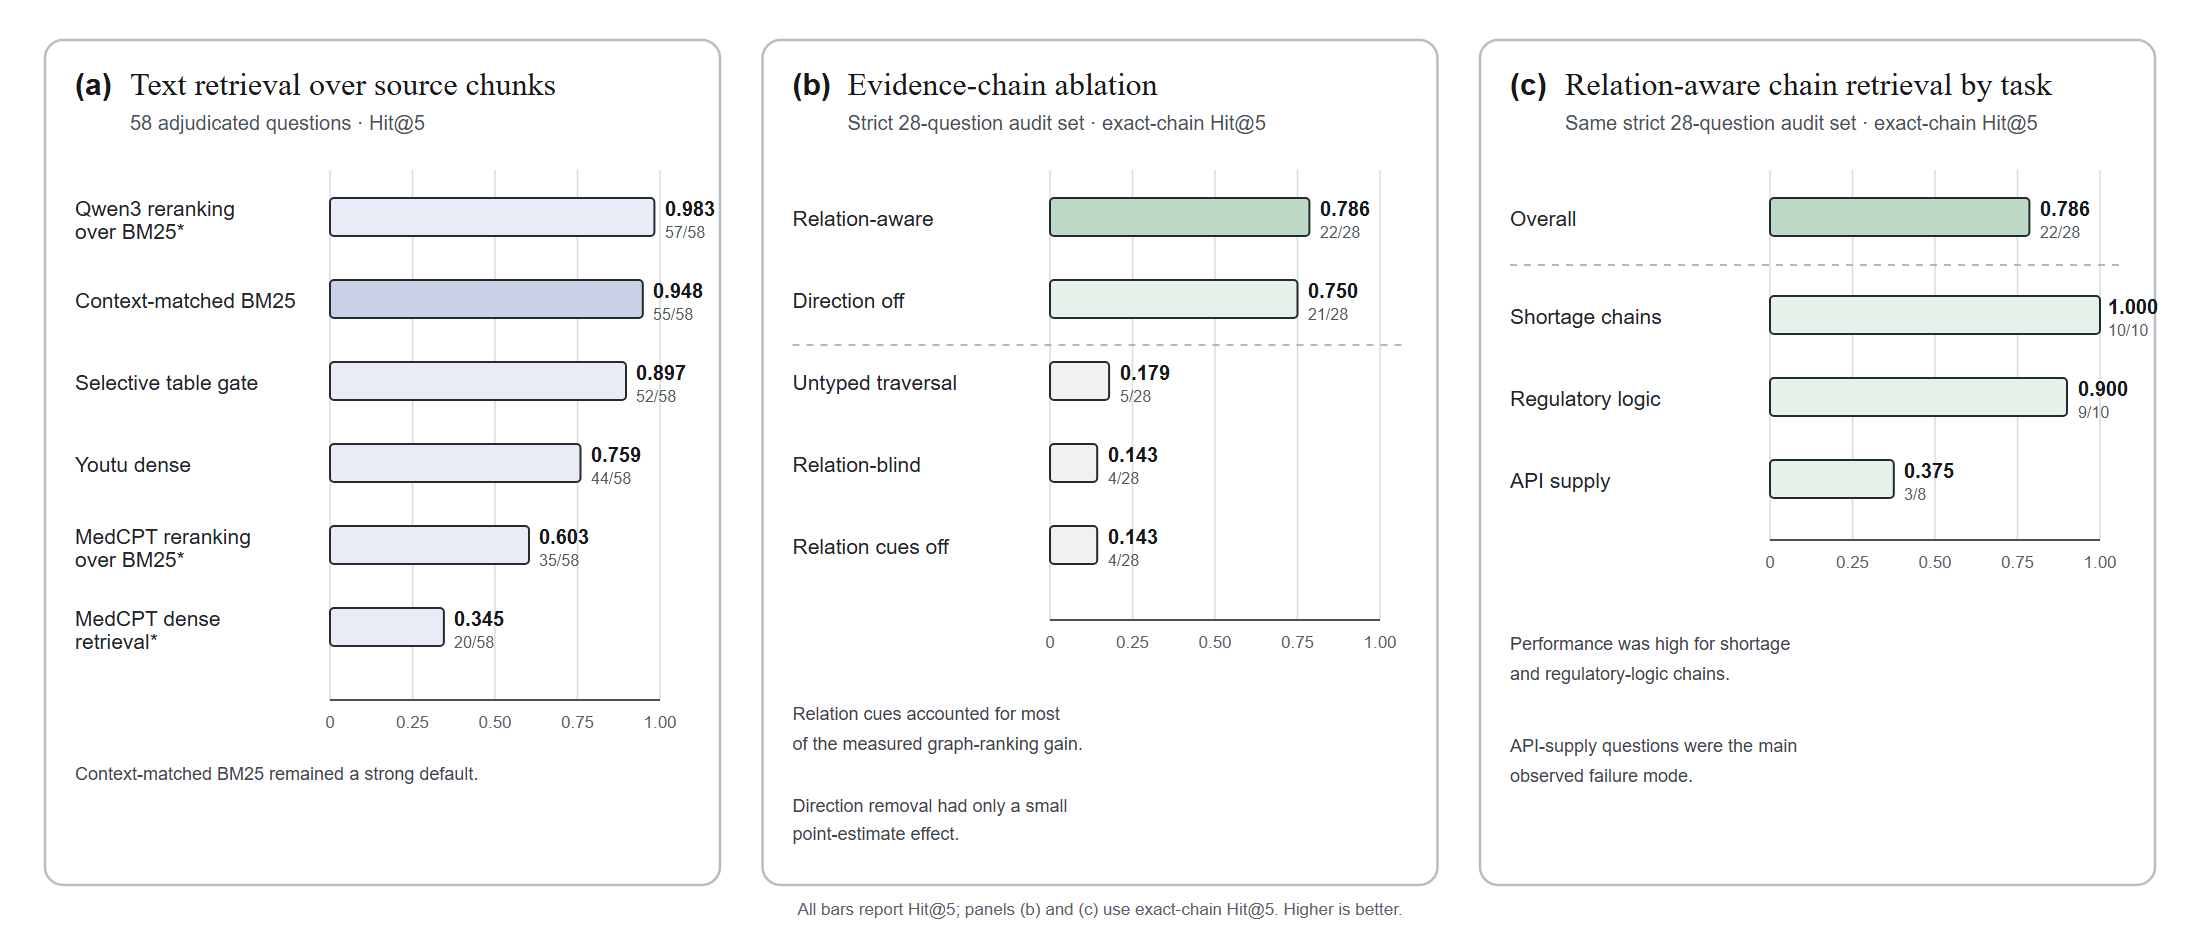
\includegraphics[width=\linewidth]{figures/retrieval_findings_summary.png}
  \caption{Summary of source-chunk and evidence-chain retrieval results. (a) Hit@5 on 58 adjudicated text questions. Asterisks mark feedback-motivated post hoc extensions evaluated under subsequently locked, unchanged inference protocols after the Gold set had been observed; they are interpreted as boundary analyses. The 95\% paired-bootstrap interval for the Qwen3--BM25 Hit@5 difference included zero. The darker lavender fill identifies the primary BM25 baseline. (b) Exploratory exact-chain Hit@5 for the relation-aware method and its controls on the strict 28-question audit set. (c) Exploratory exact-chain Hit@5 for the complete relation-aware method by task. Two questions with non-unique frozen-graph paths were retained in the 30-question audit record but excluded from strict exact-chain evaluation. Values show proportions and exact hit counts.}
  \label{fig:retrieval-findings}
\end{figure}
